\documentclass[12pt]{article}

\usepackage{sbc-template}
\usepackage{graphicx,url}
\usepackage[utf8]{inputenc}
\usepackage[brazil]{babel}
\usepackage{subcaption}
     
\sloppy

\title{Análise de Escalabilidade Horizontal em um~\emph{cluster}  Hbase}

\author{Cedryk Augusto dos Santos~\inst{1}, Bruno Santos de Lima~\inst{1}, Leandro Ungari Cayres~\inst{1},\\Rogério Eduardo Garcia~\inst{1}, Celso Olivete Junior~\inst{1}, Danilo Medeiros Eler~\inst{1},\\ Ronaldo Celso Messias Correia~\inst{1}}

\address{Faculdade de Ciências e Tecnologia -- Universidade Estadual Paulista (UNESP)\\
  Presidente Prudente -- SP -- Brasil
  \email{cedrykaugusto@gmail.com,\{bruno.s.lima,leandro.ungari,rogerio.garcia,celso.olivete,danilo.eler,ronaldo.correia\}@unesp.br}
}

\begin{document} 

\maketitle

%Resumo maximo 10 linhas.
%Se o artigo estiver em português o abstract deve estar localizado antes do resumo.

\begin{abstract}
\textbf{NoSQL Databases facilitate horizontal scheduling, allowing the distribution of resources with the addition of nodes. This work evaluates the potential of horizontal scheduling of an HBase database through a benchmarking in several scenarios, setting an ideal scenario, in order to verify the efficiency and availability of applications regardless of the demand for storage, operations and addition nodes. The results show that scalability is more evident, except in scan operations, in sets of 100,000 and 1,000,000 records of 1KB each, increasing the number of nodes from 1 to 2 and from 2 to 3. In search operations, there is no improvement in performance from the insertion of nodes.}
\end{abstract}
     
\begin{resumo} 
Os Bancos de Dados \emph{NoSQL} facilitam escalonamento horizontal, permitindo a distribuição de recursos com a adição de nós. Este trabalho avalia o potencial do escalonamento horizontal de um~\emph{cluster} do Banco de Dados Hbase, através de um \emph{benchmarking} em diversos cenários, configurando um cenário ideal, de modo a verificar a eficiência e disponibilidade de aplicações independentemente da demanda de armazenamento, operações e adição nós. Os resultados demonstram que a escalabilidade é mais evidente, exceto em operações \emph{scan}, em conjuntos de 100.000 e 1.000.000 de registros de 1KB cada, no aumento do número de nós de 1 para 2 e, de 2 para 3. Nas operações de busca, não há melhora no desempenho a partir da inserção de nós.
\end{resumo}


\section{Introdução}
\label{sec:introducao}
 
Um dos grandes desafios computacionais consiste no armazenamento, recuperação e disponibilidade de dados de modo eficiente. Durante muitos anos, a solução para a maioria dos problemas dessa área foram os Sistemas Gerenciadores de Banco de Dados Relacionais (SGBDR), que garantem o conjunto de propriedades ACID (Atomicidade, Consistência, Isolamento e Durabilidade). Contudo, os SGBDR’s não satisfazem as necessidades de sistemas no âmbito de~\emph{Big Data}.%~\cite{brito2010bancos}.
 
O conceito de \textit{Big Data} refere-se ao grande volume de dados gerados em diversos domínios de aplicação~\cite{han2011survey}. A partir desse conceito, identificou-se que a tecnologia relacional possui fragilidade no tratamento de dados classificados como semiestruturados e não estruturados, além de dificuldade de implementação distribuída, de modo a atender as propriedades ACID~\cite{aparicio:2016}. A complexidade lógica existente na modelagem relacional somada ao alto volume de dados mostrou-se um problema, visto que pode propiciar \textit{deadlocks}, além de problemas de concorrência, lentidão na leitura e escrita dos dados~\cite{han2011survey}. Como alternativa surgiram os Bancos de Dados \textit{NoSQL}, os quais atuam de modo mais eficiente com o armazenamento e manipulação de grande volume de dados, possibilitando escalar horizontalmente operações por diversos servidores, além de prover maior flexibilidade~\cite{ramesh:2016}.

Neste contexto, o objetivo deste trabalho consiste em verificar o potencial desse novo paradigma de armazenamento e recuperação de dados utilizando computação distribuída, de modo a criar um cenário, em que aplicações e serviços se mantenham eficientes e disponíveis independentemente do tamanho da demanda de armazenamento e consultas, somente através da adição de novos nós ao ambiente distribuído. Desse modo, através de um experimento foi avaliada a escalabilidade horizontal do Banco de Dados Hbase, foi executado um~\emph{benchmarking} com operações~\emph{read},~\emph{write},~\emph{scan} e~\emph{read-modify-write} utilizando o \textit{framework}~\emph{Yahoo! Cloud Serving Benchmark} (YCSB) a partir da inserção de novos nós ao sistema e crescimento do conjunto de dados.

O ambiente de desenvolvimento Hadoop foi criado pela~\emph{Apache Foundation} e reúne ferramentas de manipulação~\emph{Big Data}, envolvendo o Banco de Dados Hbase, o sistema de arquivos distribuídos~\emph{Hadoop Distributed File System} (HDFS) e o modelo de suporte a programação paralela em grandes coleções de dados chamado MapReduce~\cite{hadoophbase}. O Banco de Dados Hbase permite o processamento distribuído por meio de~\emph{clusters}, atuando sobre o HDFS de modo a agregar à ferramenta capacidades semelhantes ao BigTable~\cite{chang2008bigtable} e alta tolerância a falhas ao armazenar grandes quantidades de dados esparsos~\cite{hadoophbase}.

Além dessa introdução, este trabalho está organizando do seguinte modo: Na Seção~\ref{sec:fundamentacao} são apresentados conceitos de escalabilidade em banco de dados e as ferramentas utilizadas; A Seção~\ref{sec:relacionados} expõe os trabalhos relacionados; A Seção~\ref{sec:conf-experimento} apresenta a configuração do experimento abordando os cenários de testes utilizados; A Seção~\ref{sec:resultados} exibe a análise dos resultados obtidos; Por fim, a Seção~\ref{sec:finais} apresenta as considerações finais e indica trabalhos futuros.

\section{Fundamentação Teórica}
\label{sec:fundamentacao}

\subsection{Escalabilidade em Banco de Dados}
\label{subsec:escalabilidade}

Escalabilidade é a capacidade de expandir os recursos (armazenamento e processamento) de um sistema~\cite{elmasri2010fundamentals}. Um Banco de Dados escalável possui a capacidade de manipular quantidades de dados cada vez maiores e garantir a disponibilidade do sistema. Existem duas abordagens para escalabilidade:~\emph{Vertical} e~\emph{Horizontal}.

A~\emph{Escalabilidade Vertical}, consiste em adicionar mais recursos (CPU / Memória RAM / Disco Rígido) ao servidor. Prove menor consumo de energia, menores problemas de arrefecimento e implementação facilitada. Suas desvantagens são: custo extremamente superior a escalabilidade horizontal, possibilidade de interrupção do serviço por falha devido a um único servidor~\cite{hwang2014scale}. Em contraponto, na~\emph{Escalabilidade Horizontal}, os recursos são distribuidos em diferentes servidores, em geral máquinas simples, com o propósito de redução de custos. Existe garantia de recuperação em caso de falhas, devido a presença de redundância de dados e processos em diversos nós. Essa arquitetura é muito semelhante em diversos Banco de Dados \textit{NoSQL}~\cite{hwang2014scale}.

\subsection{Apache Hadoop}
\label{subsection:hadoop}

A biblioteca de softwares Apache Hadoop consiste em um (\textit{framework}) para processamento distribuído de grande volume de dados em~\emph{clusters}. Utiliza o modelo de programação simples \emph{MapReduce}, projetado para escalonamento horizontal, oferecendo alta disponibilidade e recuperação de falhas~\cite{hadoophbase}.

Um~\emph{cluster} Hadoop opera sob a arquitetura mestre/escravo -- Figura~\ref{figure:hadoop}. Existem cinco processos O~\emph{NameNode} e o~\emph{JobTraker} são processos executados pelo nó-mestre, enquanto~\emph{SecondaryNameNode} pelo nó-mestre alternativo, em caso de falha. O~\emph{DataNode} e~\emph{TaskTraker} atuam como processos escravos de múltiplas instâncias. %Os processos~\emph{NameNode},~\emph{SecondaryNameNode} e~\emph{DataNode} fazem parte da execução do sistema de arquivos HDFS, enquanto~\emph{JobTraker} e~\emph{TaskTraker} parte da execução MapReduce~\cite{goldman2012apache}.

\begin{figure}[!ht]
\centering
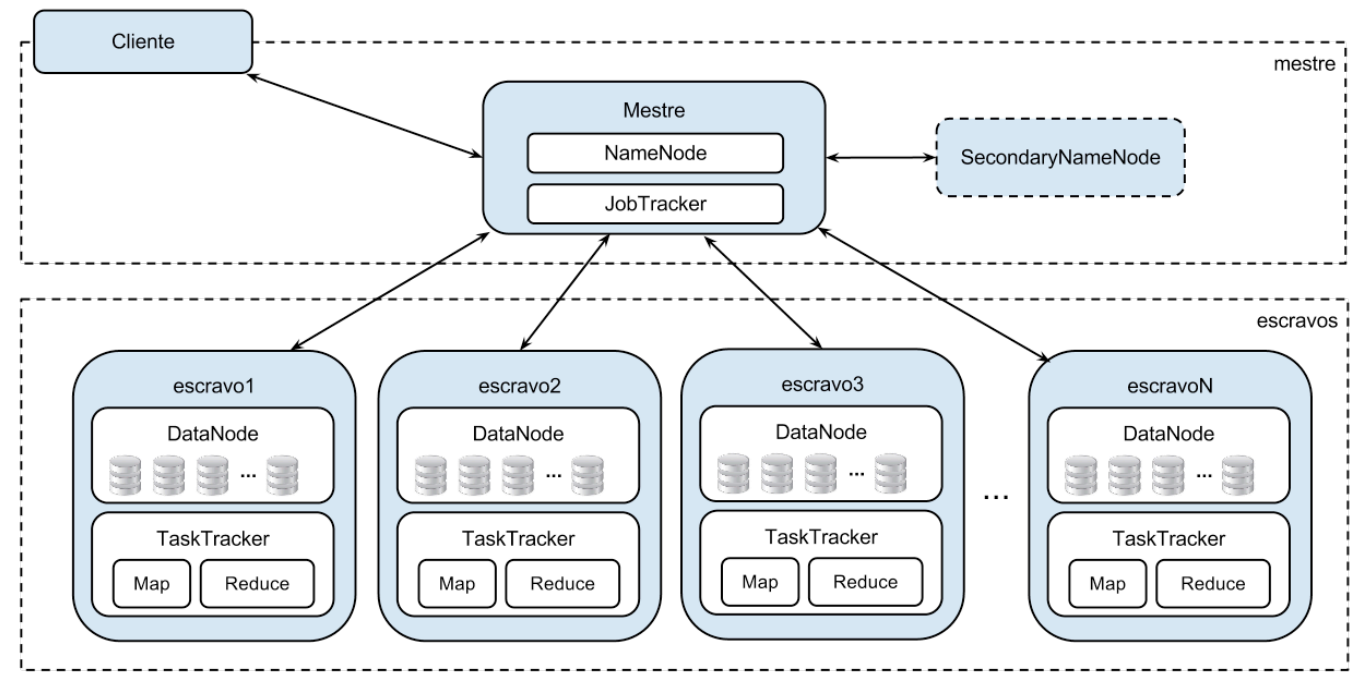
\includegraphics[width=0.7\textwidth]{images/hadoop.png}
\caption{Estrutura dos processos do Hadoop~\cite{goldman2012apache}.}
\label{figure:hadoop}
\end{figure}

%\subsection{HDFS}
%\label{subsec:hdfs}

%O HDFS consiste em um sistema de arquivos distribuídos projetado para ser tolerante a falhas, voltado para~\emph{hardwares} de baixo custo e aplicações com grande volume de dados. Assim como um sistema de arquivos, o HDFS fornece operações de armazenamento, organização, nomeação, atribuição de permissões de acesso, compartilhamento e recuperação de forma transparente ao usuário, porém, o diferencial está no armazenamento dos arquivos, os quais compartilhados por máquinas remotas ligadas em rede.

%O processo~\emph{NameNode} tem responsabilidade pela abertura, fechamento ou renomeação de arquivos e diretórios; realizar o controle de acesso dos arquivos, armazenar metadados, coordenar a fragmentação dos arquivos em blocos, assim como a distribuição dos mesmos dentro dos processos~\emph{DataNodes}. Os processos~\emph{DataNode} tem a tarefa de armazenar os dados, responder as solicitações de leitura e escrita dos clientes e aplicações, criar, remover ou replicar blocos sob orientação do~\emph{NameNode}. Além de armazenar, os~\emph{DataNode} precisam se comunicar constantemente com o~\emph{NameNode} para manter o mapeamento dos blocos atualizado e livre de falhas~\cite{hadoophdfs}.

\subsection{HBase}
\label{subsec:hbase}

O Hbase é um Banco de Dados~\textit{NoSQL}, distribuído, tolerante a falhas, de código aberto e altamente escalável. Tem como foco aplicações que necessitam de leitura e escrita de acesso aleatório com tempo constante em grandes volumes de dados~\cite{hadoophbase}. O projeto foi inspirado no \textit{BigTable} da Google, ambos utilizam o modelo de dados orientado a colunas. Esse não possui nenhuma linguagem de consulta estruturada, porém fornece uma API Java que possibilita realizar operações básicas como~\emph{put},~\emph{get},~\emph{update} e~\emph{delete}. Possibilita também o uso da função~\emph{scan}, para selecionar quais as colunas a serem retornadas ou o número de versões de cada célula. Consultas mais complexas ficam a cargo de jobs do MapReduce~\cite{cunha2015column}.

Os dados do HBase são armazenados como arquivos do HDFS. O HDFS consiste em um sistema de arquivos distribuídos projetado para ser tolerante a falhas, voltado para~\emph{hardwares} de baixo custo e aplicações com grande volume de dados. Dessa forma, os servidores escravos (~\emph{region servers}) são dispostos nos nós que executam os processos~\emph{DataNode} do HDFS provendo localidade nos dados que transitam de um para o outro.

\subsection{Yahoo! Cloud Serving Benchmark}
\label{subsec:ycsb}

O YCSB (\emph{Yahoo! Cloud Serving Benchmark}) é um \textit{framework} de código-aberto para apoio a~\emph{benchmarking} de diferentes Bancos de Dados distribuídos, a qual permite a extensão para Banco de Dados não implementados previamente~\cite{cooper2010benchmarking}. O YCSB possibilita a avaliação de duas camadas de \textit{benchmark}: performance e escalabilidade. Em performance, mede-se a latência (tempo de execução) das requisições, em escalabilidade é medido o impacto na performance quando o número de servidores do sistema cresce~\cite{cooper2010benchmarking}.

O \textit{framework} possui um conjunto de~\emph{workloads} denominado~\emph{Core Package} e uma aplicação chamada YCSB \textit{Client}. As~\emph{workloads} consistem de combinações de operações de leitura e escrita, na execução de uma~\emph{workload}, o YCSB \textit{Client} cria um conjunto de dados e submete as requisições ao banco de dados~\cite{cooper2010benchmarking}.

\section{Trabalhos Relacionados} 
\label{sec:relacionados}

Na literatura alguns trabalhos relacionados também avaliam o desempenho da ferramenta Hbase por meio de \textit{benchmarking} com outros Bancos de Dados ou ainda colocando alguma condição sobre os dados a serem manipulados.

Em seu estudo, \cite{jogi2016performance} realizam a comparação MySQL com Cassandra e Hbase em operações~\emph{heavy~\emph{write}}. Foi elaborada uma aplicação~\emph{web} REST (\emph{Representacional State Transfer}) para recebimento dos dados e armazenamento no Banco de Dados. Em conclusão, o Cassandra apresentou melhor desempenho entre os três bancos quanto a velocidade de escrita, enquanto o Hbase foi duas vezes mais rápido que o MySQL. Para os autores~\cite{jogi2016performance}, o comportamento do Cassandra ocorre devido a incorporação de características do \emph{BigTable} do Google e do DynamoDB. \cite{swaminathan2016quantitative} conduziram uma análise de escalabilidade nos Bancos de Dados: Hbase, Cassandra e MongoDB. Para isso foi utilizado o \textit{framework} YCSB com diferentes cargas de trabalho e conjunto de dados, no intuito de evidenciar as vantagens e desvantagens de cada ferramenta para um cenário específico.

Segundo~\cite{waage2014benchmarking}, a confiabilidade para o armazenamento ``em nuvem'' é um dos pontos chaves para adoção de tecnologias não-relacionais. Desse modo, é proposto que os dados sejam criptografados de modo prévio. Para avaliar o impacto da criptografia, foi realizado um estudo com os Bancos de Dados Cassandra e Hbase. Para tal fo utilizado o \emph{framework} YCSB em que~\emph{workloads} foram aplicadas a dados não-encriptados e encriptados usando o algoritmo~\emph{Advanced Encryption Standard} (AES) com chaves de 128, 192 e 256 bits de comprimento. Em suma, foi relatada uma redução no desempenho médio do~\emph{cluster}, o qual é independente do tamanho da chave de encriptação.

Na apresentação do \textit{framework} YCSB,~\cite{cooper2010benchmarking} aplicaram~\emph{benchmarking} nos Banco de Dados: Cassandra, Hbase, Yahoo!’s PNUTS e o Sharded MySQL, para exemplificar o uso do \textit{framework} de maneira prática. A partir de testes de performance e escalabilidade, observaram que o Cassandra e Hbase apresentam maior latência para operações~\emph{read} e menor latência para operações~\emph{update} e~\emph{write} em relação ao PNUTS e MySQL, enquanto o PNUTS e Cassandra melhor escalabilidade, em detrimento ao HBase, quando o número de servidores no~\emph{cluster} aumenta proporcionalmente a carga de trabalhos.

Diferentemente dos estudos presentes na literatura, este trabalho avalia o potencial do escalonamento horizontal de um~\emph{cluster} do Banco de Dados Hbase, através de um \textit{benchmarking} sobre diversos cenários, de modo a criar um cenário, em que aplicações e serviços se mantenham eficientes e disponíveis independentemente do tamanho da demanda de armazenamento e consultas. Concomitantemente, também é verificado aspectos de eficiência e disponibilidade.

\section{Configuração do Ambiente de Experimentação}
\label{sec:conf-experimento}

Os testes foram executados em um~\emph{cluster} composto por 7 computadores todos utilizando o Sistema Operacional Linux CentOS 6.6, sendo um deles o nó mestre denominado hpcdmc e os seis caracterizados como nós escravos denominados de n01 a n06. \textbf{Configuração do nó mestre (hpcdmc):} 2x Processador Intel Xeon E5-2620 2.0GHz 6 núcleos; 4x Memória Ram Kingston DDR3 8GB 1333MHz; 8x Sata3 de 2TB. \textbf{Configuração dos nós escravos e cliente (n01 a n06):} 2x Processador Intel Xeon E5-2690 2.90GHz 8 núcleos; 4x Memória Ram Kingston DDR3 8GB 1600MHz; 8x Sata3 de 500GB e 16MB de cache.

%Configuração do nó mestre (hpcdmc):
%\begin{itemize}
%\item Sistema Operacional Linux CentOS 6.6
%\item 2x Processador Intel Xeon E5-2620 2.0GHz 6 núcleos
%\item 4x Memória Ram Kingston DDR3 8GB 1333MHz
%\item 8x Sata3 de 2TB
%\end{itemize}
%Configuração dos nós escravos e cliente (n01 a n06):
%\begin{itemize}
%\item Sistema Operacional Linux CentOS 6.6
%\item 2x Processador Intel Xeon E5-2690 2.90GHz 8 núcleos
%\item 4x Memória Ram Kingston DDR3 8GB 1600MHz
%\item 8x Sata3 de 500GB e 16MB de cache
%\end{itemize}
Para a execução do experimento foram utilizados os softwares: Hadoop 2.7.3; HBase 1.2.4; ZooKeeper 3.4.10; YCSB 0.12.0. As versões dos softwares utilizados foram escolhidas por serem as mais estáveis e atuais, até o momento do desenvolvimento deste trabalho, de acordo com as informações obtidas pela documentação dos desenvolvedores de cada aplicação.

Primeiramente foram organizados cinco cenários de organização para o~\emph{cluster}, nos quais foram executados os testes iniciais. Com base nesses cinco cenários e nos testes realizados foi analisado a melhor alternativa para a implementação do~\emph{cluster} e avaliar sua escalabilidade, ou seja, como serão dispostos os processos cliente, mestre e escravo, e assim foi idealizado e avaliado o sexto cenário.

Para os cinco primeiros cenários foram executados os testes em um ambiente pseudo distribuído, com duas~\emph{workloads}: 100\%~\emph{write} e 100\%~\emph{read} -- 100.000 registros, tendo cada registro 1KB e distribuição uniforme. Cada teste sobre uma~\emph{workload} foi executado 3 vezes para uma dada quantidade de~\emph{threads} do YCSB \textit{Client}, foi obtido a média da latência (tempo de execução em milissegundos) e do desempenho médio (operações/segundo) para obter o resultado final do teste.

Nos testes executados no sexto cenário, configurado de acordo com as conclusões obtidas nos testes dos cenários anteriores, é analisada a escalabilidade do HBase em um~\emph{cluster} totalmente distribuído, sendo esse, o foco principal do trabalho. Cada teste sobre uma~\emph{workload} também foi executado 3 vezes sendo o resultado final a média das saídas. A seguir são descritas a organização de cada um dos cenários:

\begin{figure}
	\centering
	\hspace{0.2cm}
    \begin{subfigure}{0.2\textwidth}
    	\centering
        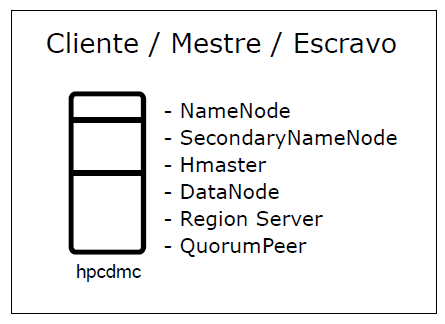
\includegraphics[width=1.0\textwidth]{images/cenario-1.png}
        \caption{Cenário 1}
        \label{figura2a}
    \end{subfigure}
    \hspace{0.3cm}
    \begin{subfigure}{0.3\textwidth}   
    	\centering
        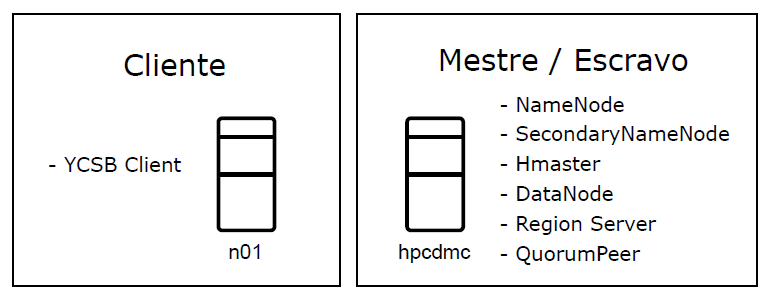
\includegraphics[width=1.1\textwidth]{images/cenario-2.png}
        \caption{Cenário 2}%
        \label{figura2b}
    \end{subfigure}
    \hspace{0.4cm}
    \begin{subfigure}{0.3\textwidth}
    	\centering
        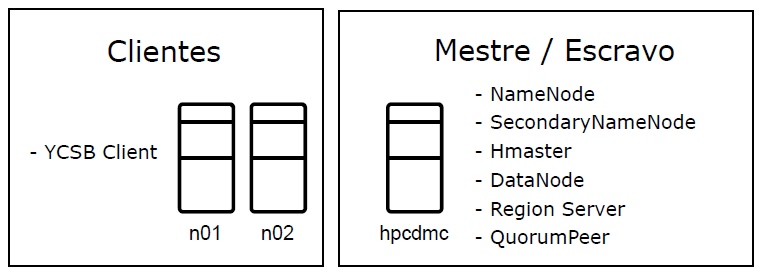
\includegraphics[width=1.1\textwidth]{images/cenario-3.png}
        \caption{Cenário 3}
        \label{figura2c}
    \end{subfigure}
    \medskip
    \begin{subfigure}{0.3\textwidth}   
    	\centering
        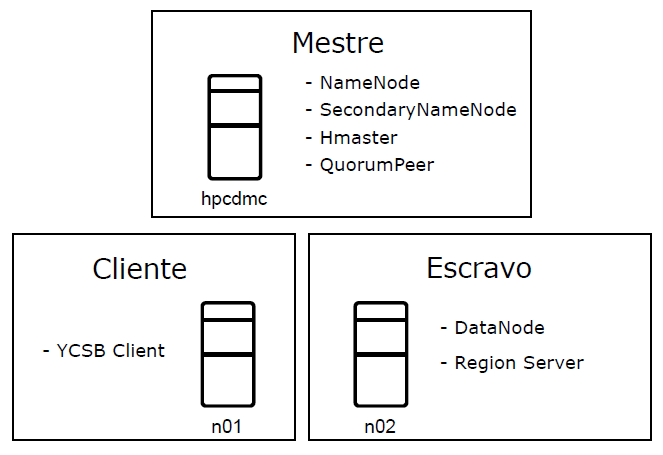
\includegraphics[width=1.0\textwidth]{images/cenario-4.png}
        \caption{Cenário 4}%
        \label{figura2d}
    \end{subfigure}
    \begin{subfigure}{0.3\textwidth}
    	\centering
        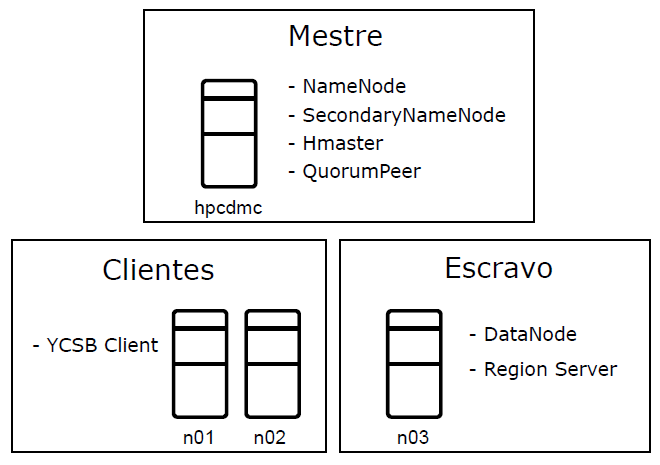
\includegraphics[width=1.0\textwidth]{images/cenario-5.png}
        \caption{Cenário 5}
        \label{figura2e}
    \end{subfigure}
    \begin{subfigure}{0.35\textwidth}   
    	\centering
        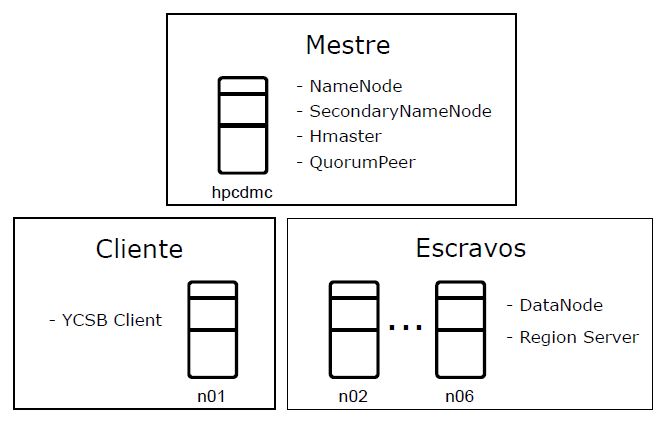
\includegraphics[width=1.0\textwidth]{images/cenario-6.png}
        \caption{Cenário 6}%
        \label{figura2f}
    \end{subfigure}
    \caption{Configuração dos seis cenários de testes.}
\end{figure}

%\subsection{Cenário 1}
\textbf{Cenário 1:} O~\emph{cluster} é configurado de modo pseudo distribuído, ou seja, os processos são executados como se houvesse uma distribuição entre máquinas em redes, porém estão todos no mesmo nó. Dessa forma, os processos mestre e escravo do Hadoop e HBase, os processos do ZooKeeper e do YCSB \emph{Client} são executados todos no hpcdmc~--~Figura~\ref{figura2a}.

%\subsection{Cenário 2}
\textbf{Cenário 2:} Considerando que a execução de todos os processos mestre e escravo junto com o YCSB \emph{Client} pode comprometer a quantidade de requisições enviadas ao banco, alocou-se o YCSB em um nó separado para verificar essa hipótese. Dessa forma, os processos meste e escravo do Hadoop e HBase e os processos do ZooKeeper continuaram a ser executados no hpcdmc, mas o processo YCSB \emph{Client} foi executado no nó n01~--~Figura~~\ref{figura2b}.

%\subsection{Cenário 3}
\textbf{Cenário 3:} Dada a limitação do número de~\emph{threads} do YCSB \emph{Client} que podem ser executadas no n01, pelo número de núcleos do processador, no cenário 3 a execução da~\emph{workload} foi dividida entre nós n01 e n02. Cada nó foi encarregado pela metade dos registros e metade do número de~\emph{threads} do YCSB \emph{Client} total do teste. Exemplo: na execução da~\emph{workload} 100\%~\emph{read} e 64~\emph{threads}, cada nó gerou 50.000 requisições~\emph{read} com 32~\emph{threads} ativas no YCSB. A saída de cada teste foi a soma do desempenho médio (operações/segundo) e a maior latência (tempo de execução em milissegundos) de ambos. O hpcdmc permaneceu pseudo distribuído~--~Figura~\ref{figura2c}.

%\subsection{Cenário 4}
\textbf{Cenário 4:} Consiste na aproximação de uma situação mais adequada quanto a configuração do~\emph{cluster} , onde os processos cliente, mestre e escravo estão completamente distribuídos. O n01 é responsável pelo YCSB \textit{Client}, o hpcdmc pelos processos mestre do Hadoop, HBase e dos processos do ZooKeeper, enquanto o n02 executou os processos escravos do Hadoop e HBase~--~Figura~\ref{figura2d}.

%\subsection{Cenário 5}
\textbf{Cenário 5:} Teve como objetivo dos testes analisar se é necessário mais de um servidor gerando requisições para saturar um~\emph{cluster} completamente distribuído. Assim, o n01 e n02 dividiram a execução das~\emph{workloads}, o hpcdmc foi responsável pelos processos mestre do Hadoop, HBase e os processos do ZooKeeper e o n03 executou os processos escravos do Hadoop e HBase~--~Figura~\ref{figura2e}.

%\subsection{Cenário 6}
\textbf{Cenário 6:} Os resultados dos testes realizados nos cenários anteriores apoiam as decisões quanto a estrutura geral do cenário 6~--~Figura~\ref{figura2f}. Foram executadas as~\emph{workloads}:~\emph{write},~\emph{read} e~\emph{scan}, variando entre 1.000, 10.000, 100.000 e 1.000.000 registros com tamanho igual a 1KB e com distribuição uniforme, variando o número de escravos de 1 a 5 e o número de~\emph{threads} do YCSB \textit{Client} fixo.

\section{Resultados e Discussões}
\label{sec:resultados}

\subsection{Testes dos Cenários de 1 a 5}

Os cenários 1 e 2 demonstraram um crescimento no desempenho médio do~\emph{cluster} nas execuções com até 64~\emph{threads} -- Figuras~\ref{figura11} e~\ref{figura13}. No cenário 1, entre 1 e 64~\emph{threads} ocorreu um aumento de aproximadamente 90\% no desempenho médio, enquanto no cenário 2 ocorreu, para a mesma quantidade de~\emph{threads}, um aumento de aproximadamente 93\%.

Na instanciação de mais de 64~\emph{threads}, no cenário 1 observa-se queda no desempenho médio de aproximadamente 5\% nos testes com 128~\emph{threads} e, no cenário 2, também quedas nas execuções de 128, 256 e 512~\emph{threads}, sendo a mais expressiva de aproximadamente 10\% nas execuções com 256~\emph{threads}. Ambas as porcentagens foram calculadas comparando os resultados às execuções com 64~\emph{threads}.

Da mesma forma, observa-se queda na latência nos testes dos cenários 1 e 2 até as execuções com 64~\emph{threads} -- Figuras~\ref{figura12} e~\ref{figura14}. Dado a medida que o desempenho médio aumenta, ou seja, o~\emph{cluster} executa mais operações por segundo, o tempo de execução do teste diminui. Para o cenário 1, a queda da latência entre as execuções com 1 e 64~\emph{threads} foi de aproximadamente 90\% e, para o cenário 2 de aproximadamente 93\%.

Constata-se que o desempenho máximo do~\emph{cluster} foi obtido para os dois cenários nas execuções do YCSB \textit{Client} com 64~\emph{threads}, a partir do cenário 3 foram executados apenas os testes de 64 a 512~\emph{threads}, de modo a observar se esses resultados foram ótimos locais ou globais. Os testes do cenário 1, para 256 e 512~\emph{threads} não puderam ser executados por estouro da pilha de memória do nó hpcdmc ao executar o YCSB \textit{Client} já que, além do YCSB \textit{Client} o nó hpcdmc também estava executando os processos mestre e escravo do Hbase e Hadoop e os processos do ZooKeeper.

A análise dos resultados obtidos pela execução testes com a~\emph{workload} 100\%~\emph{write} -- 100.000 registros, mostrou que o melhor desempenho médio foi alcançado pelo cenário 5 para as execuções com 64 e 128~\emph{threads}, sendo maior que os resultados dos cenários 4, 3, 2 e 1 aproximadamente 5,7\%, 19,4\%, 25,4\% e 50,3\% nas execuções com 64 \emph{threads} e, 8,2\%, 27,4\%, 28,6\% e 54\% nas execuções com 128~\emph{threads}, respectivamente. Para as execuções com 256 e 512~\emph{threads} o melhor desempenho médio foi obtido pelo cenário 4 sendo maior que os cenários 5, 3 e 2 aproximadamente 0,8\%, 22,6\% e 35,6\% nas execuções com 256~\emph{threads} e, 58\%, 19,9\% e 21,2\% nas execuções com 512~\emph{threads}respectivamente.

\begin{figure*}
    \centering
    \begin{subfigure}[b]{0.49\textwidth}
        \centering
        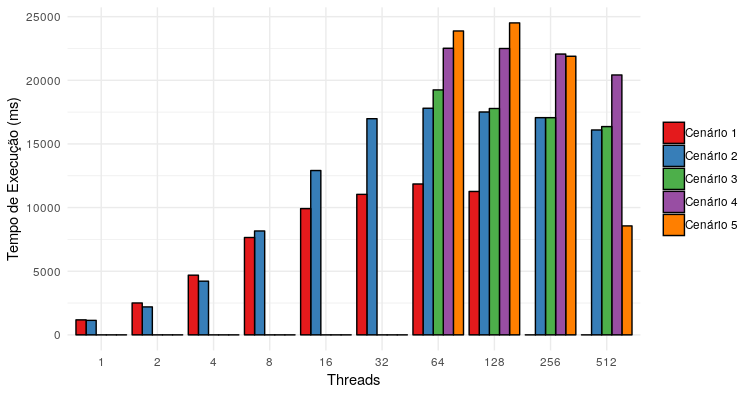
\includegraphics[width=\textwidth]{images/figura11}
        \caption{Desempenho médio}
        \label{figura11}
    \end{subfigure}
        \hfill
    \begin{subfigure}[b]{0.49\textwidth}  
        \centering 
        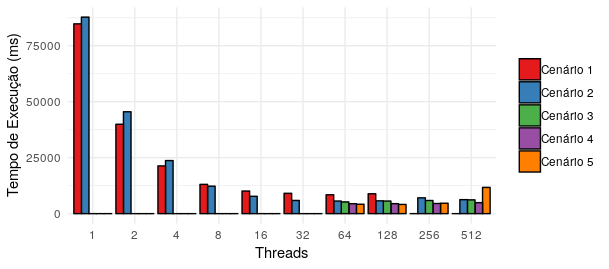
\includegraphics[width=\textwidth]{images/figura12}
        \caption{Latência}%
        \label{figura12}
    \end{subfigure}
    \caption{\emph{Workload} 100\%~\emph{write} 100.000 registros nos cenários de 1 a 5.}
\end{figure*}

O cenário 5 apresentou esse desempenho pois o~\emph{cluster} foi completamente distribuído, então os processos mestres e escravo do Hbase e Hadoop, processos do ZooKeeper e YCSB não concorreram por recursos de uma mesma máquina uns com os outros. O mesmo ocorreu no cenário 4, mas a divisão da execução das~\emph{workloads} entre o n01 e n02 apresentou uma pequena melhora no cenário 5 no desempenho do~\emph{cluster} executando o YCSB com 64 e 128~\emph{threads}, já nas execuções com 256 e 512~\emph{threads} tal divisão sobrecarregou demais o n03 fazendo com que o desempenho médio diminuísse e a latência aumentasse, tornando os resultados do cenário 4 melhores.

A partir dos testes da~\emph{workload} 100\%~\emph{write} -- 100.000 registros, pode-se concluir que o cenário 5, para execuções com 64 e 128~\emph{threads} obteve uma execução mais rápida que os testes dos cenários 4, 3, 2 e 1 aproximadamente 5,6\%, 19,7\%, 25,4\% e 50,2\% com 64~\emph{threads} e, 7,8\%, 27\%, 28,1\% e 53,7\% com 128~\emph{threads} respectivamente. Enquanto que para as execuções com 256 e 512~\emph{threads} o cenário 4 teve uma execução mais rápida que os testes dos cenários 5, 3 e 2 aproximadamente 2,4\%, 22,8\% e 35,8\% com 256 \emph{threads} e, 95,8\%, 20,3\% e 21,5\% com 512~\emph{threads} -- Figura~\ref{figura12}.

Os resultados dos testes da~\emph{workload} 100\%~\emph{read} -- 100.000 registros, para todos os números de~\emph{threads} o cenário 5 obteve o melhor desempenho médio sendo maior que os resultados dos cenários 4, 3, 2 e 1 aproximadamente 26,8\%, 22,2\%, 48,3\% e 62,6\% nas execuções com 64~\emph{threads} e, 26,9\%, 44,3\%, 45,7\% e 64,4\% nas execuções com 128~\emph{threads} respectivamente. E maior que os resultados dos cenários 4, 3 e 2 aproximadamente 28,4\%, 23\% e 50,4\% nas execuções com 256~\emph{threads} e, 26,5\%, 18,2\% e 47,3\% nas execuções com 512~\emph{threads} respectivamente.

Para as operações de leitura especificadas na~\emph{workload} 100\%~\emph{read}, a divisão de requisições entre o n01 e n02 não sobrecarregou o n03 para execuções com 256 e 512 \emph{threads} como nos testes da~\emph{workload} 100\%~\emph{write}, então o cenário 5 obteve os melhores resultados para cada execução entre 64 e 512~\emph{threads}. Os testes do cenário 3, que também dividiram as requisições entre o n01 e n02 obtiveram os segundos melhores resultados para cada execução entre 64 e 512~\emph{threads}. Portanto para operações de leitura, o~\emph{cluster} é mais eficiente, considerando o desempenho médio e a latência, se as requisições são realizadas de mais de um cliente -- Figura~\ref{figura13}.

\begin{figure*}
    \centering
    \begin{subfigure}[b]{0.49\textwidth}   
        \centering 
        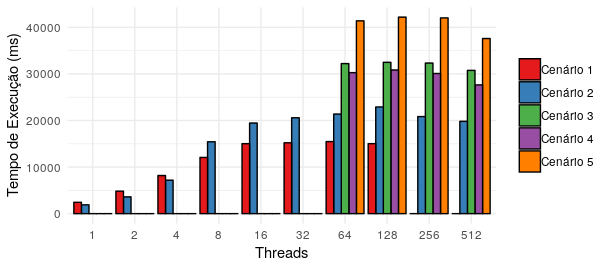
\includegraphics[width=\textwidth]{images/figura13}
        \caption{Desempenho médio}
        \label{figura13}
    \end{subfigure}
    \begin{subfigure}[b]{0.49\textwidth}   
        \centering 
        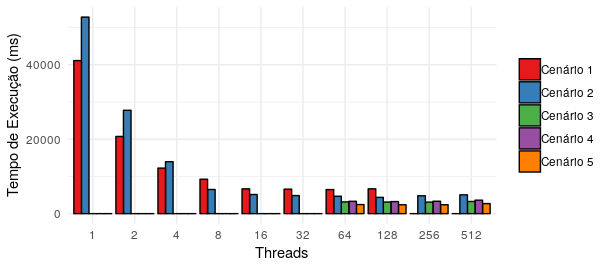
\includegraphics[width=\textwidth]{images/figura14}
        \caption{Latência}
        \label{figura14}
    \end{subfigure}
    \caption{\emph{Workload} 100\%~\emph{read} 100.000 registros nos cenários de 1 a 5.}
\end{figure*}

Na~\emph{workload} 100\%~\emph{read} -- 100.000 registros -- Figura~\ref{figura14}, a latência dos testes executados no cenário 5 foi menor que os cenários 4, 3, 2 e 1 aproximadamente 26,2\%, 22,8\%, 47,9\% e 62,3\% nas execuções com 64~\emph{threads} e, 26,6\%, 23,6\%, 45,6\% e 64,3\% nas execuções com 128~\emph{threads} respectivamente. E também, menor que os cenários 4, 3 e 2 aproximadamente 27,9\%, 22,8\% e 50\% nas execuções com 256~\emph{threads} e, 25,5\%, 17,3\% e 46.6\% nas execuções com 512~\emph{threads} respectivamente.

Observou-se também que para todos os cenários as execuções com 64 e 128~\emph{threads} são as mais altas e a variação referente a um mesmo cenário, considerando essas duas quantidades de~\emph{threads} não são expressivas, sendo de aproximadamente 1\%, para os testes da~\emph{workload} 100\%~\emph{write} e 100\%~\emph{read}, tando para o desempenho médio quanto para a latência. O aumento do número de~\emph{threads} além de 128 causou uma queda do desempenho médio nos testes dos cenários 5, 4, 3 e 2 de até 65\%, 9,3\%, 15\% e 9,6\% para os testes da~\emph{workload} 100\%~\emph{write} e, 10,9\%, 10,4\%, 5,3 e 13,5\% para os testes da~\emph{workload} 100\%~\emph{read} respectivamente. Comparando então os 5 cenários em que a execução do YCSB \emph{Client} ocorreu com 64~\emph{threads}, temos que em ambas as~\emph{workloads} 100\%~\emph{write} e 100\%~\emph{read} o cenário 5 obteve o maior desempenho médio do~\emph{cluster}, seguido pelo cenário 4 na~\emph{workload} 100\%~\emph{write} com uma diferença de aproximadamente 5,7\% e, seguido pelos cenários 3 e 4 na~\emph{workload} 100\%~\emph{read} com uma diferença de aproximadamente 22,2\% e 26,8\% respectivamente.

O cenário 4 obtive o segundo maior desempenho médio nos testes da~\emph{workload} 100\%~\emph{write} com uma diferença de menos de 6\% comparado aos resultados do cenário 5, obtiveram o terceiro maior desempenho médio nos testes da~\emph{workload} 100\%~\emph{read} com uma diferença de aproximadamente 6\% comparado com os resultados cenário 3 e, considerando também que ambos os cenários 5 e 3 utilizam 2 nós para a execução do YCSB \emph{Client}, reduzindo o número de nós disponíveis para os testes de adição de nós, a implementação do~\emph{cluster} para os testes do cenário 6 foi realizada de acordo com o cenário 4 e com 64~\emph{threads} de execução no YCSB \emph{Client}.

\subsection{Testes do Cenário 6}
\label{subsec:resultado-cenario-6}

Inicialmente, a respeito do desempenho médio~--~Figura~\ref{figura15}, a escalabilidade horizontal foi mais evidenciada quando o conjunto de dados foi igual a 1.000.000 de registros, sendo o desempenho do~\emph{cluster} com 5~\emph{region servers} maior do que os testes executados com 4, 3, 2, e 1~\emph{region servers} em aproximadamente 5,1\%, 6,5\%, 17,1\% e 47\% respectivamente. Os resultados dos testes em que o conjunto de dados foi igual a 100.000 registros também apresentou certa escalabilidade, sendo o desempenho médio com 5~\emph{region servers} maior do que o desempenho médio dos testes executados com 4, 3, 2, e 1~\emph{region servers} em aproximadamente 9,9\%, 10,4\%, 15,7\% e 43,4\% respectivamente.

\begin{figure*}[!ht]
    \centering
    \begin{subfigure}[b]{0.49\textwidth}
        \centering
        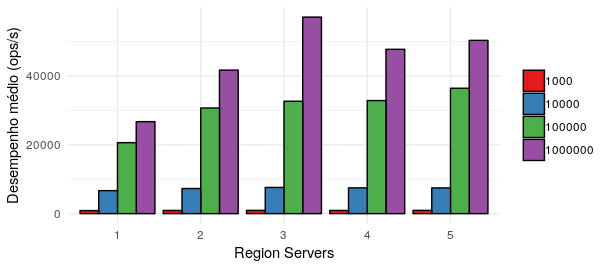
\includegraphics[width=\textwidth]{images/figura15}
        \caption{Desempenho médio}
        \label{figura15}
    \end{subfigure}
        \hfill
    \begin{subfigure}[b]{0.49\textwidth}  
        \centering 
        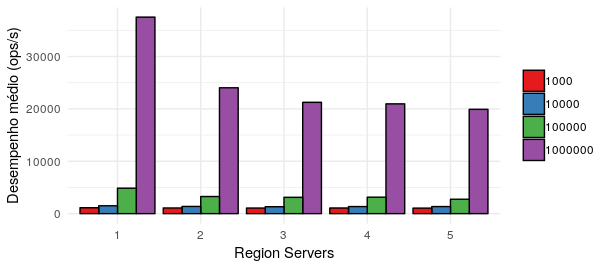
\includegraphics[width=\textwidth]{images/figura16}
        \caption{Latência}
        \label{figura16}
    \end{subfigure}
    \caption{\emph{Workload} 100\%~\emph{write} variando o tamanho do conjunto de dados e o número de~\emph{region servers} do~\emph{cluster} .}
\end{figure*}

\begin{figure*}[!ht]
    \centering
    \begin{subfigure}[b]{0.49\textwidth}
        \centering
        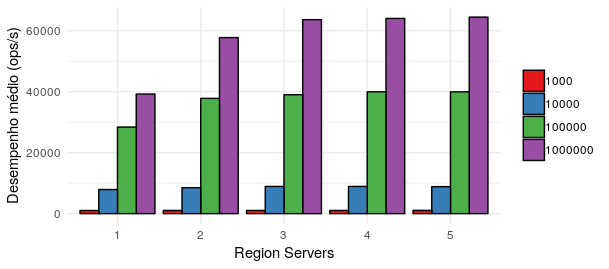
\includegraphics[width=\textwidth]{images/figura17}
        \caption{Desempenho médio}
        \label{figura17}
    \end{subfigure}
        \hfill
    \begin{subfigure}[b]{0.49\textwidth}  
        \centering 
        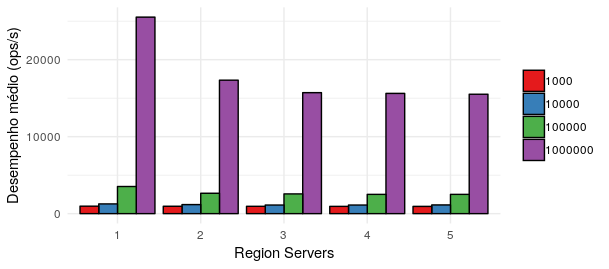
\includegraphics[width=\textwidth]{images/figura18}
        \caption{Latência}%
        \label{figura18}
    \end{subfigure}
    \caption{\emph{Workload} 100\%~\emph{read} variando o tamanho do conjunto de dados e o número de \emph{region servers} do~\emph{cluster}.}
\end{figure*}

A partir dos resultados dos testes da~\emph{workload} 100\%~\emph{write}~--~Figura~\ref{figura16}, observa-se que quando os conjunto de dados foram iguais a 1.000.000 registros obtiveram uma latência menor que os testes com 4, 3, 2 e 1 \emph{region server} em aproximadamente 5\%, 6,3\%, 17,1\% e 47\% respectivamente. Os resultados dos testes com 100.000 registros, onde a escalabilidade foi menos evidenciada, as latências tiveram poucas alterações comparados os resultados dos testes com 4, 3, 2 e 1 \emph{region server}, sendo menor em aproximadamente 12,5\%, 11,7\%, 15,9\% e 43,4\% respectivamente.

Os testes em que os conjuntos de dados foram iguais a 1.000 e 10.000 registros não tiveram alterações tão significativas no desempenho médio com a adição de novos nós, sendo a variação mais expressiva para o conjunto de dados de 1.000 registros de aproximadamente 4\% aumentando de 1 para 2~\emph{region servers}, aproximadamente 8\% para o conjunto de dados de 10.000 aumentando de 1 para 2 \emph{region servers}, considerando tanto o desempenho médio~--~Figura~\ref{figura17}, quanto a latência~--~Figura~\ref{figura18}.

%Figura ficava aqui

Para a~\emph{workload} 100\%~\emph{read}, assim como nos resultados acima, nota-se que a escalabilidade horizontal foi mais evidenciada quando o conjunto de dados foi igual a 1.000.000 de registros. Porém nas execuções com 5 \emph{region servers} só existiu alteração significativa no desempenho médio quando comparadas com as execuções com 2 e 1 \emph{region servers}, sendo maior em aproximadamente 10,4\% e 39,1\% respectivamente. Para as execuções com 4 e 3~\emph{region servers} a variação foi de menos de 1,5\%~--~Figura~\ref{figura17}. Pelos resultados dos testes com 100.000 registros, nota-se o mesmo comportamento, sendo o desempenho médio das execuções com 5~\emph{region servers} maior que os testes com 2 e 1~\emph{region servers} aproximadamente 5,4\% e 29\% respectivamente. Para as execuções com 4 e 3~\emph{region servers} a variação foi de menos de 2,4\%. Os testes em que os conjuntos de dados foram iguais a 1.000 e 10.000 registros não tiveram alterações significativas, sendo a variação mais expressiva para o conjunto de dados de 1.000 registros de menos de 1,5\% aumentando de 1 para 2~\emph{region servers} e para o conjunto de 10.000 registros de menos de 7,5\% também aumentando de 1 para 2~\emph{region servers}.

A latência dos testes da~\emph{workload} 100\%~\emph{read}~--~Figura~\ref{figura18}, também não apresentou alterações significativas para os testes cujos conjuntos de dados foram iguais 1.000.000 e 100.000 registros quando variados os~\emph{region servers} entre 3 e 5, sendo essa variação de menos de 1,3\% para ambos os conjuntos. Desta forma, os testes executados com 5~\emph{region servers} apresentaram uma latência menor que os testes com 2 e 1~\emph{region servers} em aproximadamente 10,5\% e 40,2\% com 1.000.000 de registros e, em aproximadamente 5,4\% e 29\% com 100.000 registros respectivamente. Os testes em que os conjuntos de dados foram iguais a 1.000 e 10.000 registros não tiveram alterações significativas no desempenho médio, sendo a variação de 1 para 5 \emph{region servers} de menos de 3,3\% para o conjunto de 1.000 registros e, de menos de 10,7\% para o conjunto de 10.000 registros.

\begin{figure*}[!ht]
    \centering
    \begin{subfigure}[b]{0.49\textwidth}
        \centering
        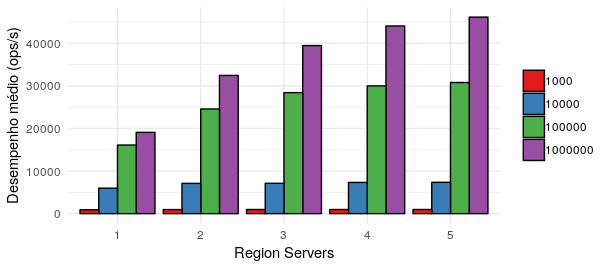
\includegraphics[width=\textwidth]{images/figura19}
        \caption{Desempenho médio}
        \label{figura19}
    \end{subfigure}
        \hfill
    \begin{subfigure}[b]{0.49\textwidth}  
        \centering 
        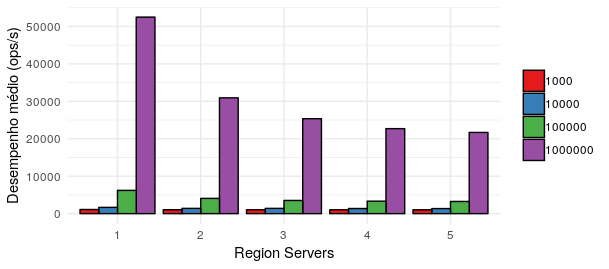
\includegraphics[width=\textwidth]{images/figura20}
        \caption{Latência}%
        \label{figura20}
    \end{subfigure}
    \caption{\emph{Workload} 100\%~\emph{read/modify/write} variando o tamanho do conjunto de dados e o número de \emph{region servers} do \emph{cluster}.}
\end{figure*}

\begin{figure*}
    \centering
    \begin{subfigure}[b]{0.49\textwidth}   
        \centering 
        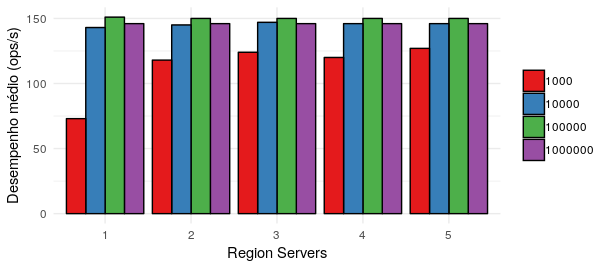
\includegraphics[width=\textwidth]{images/figura21}
        \caption{Desempenho médio}
        \label{figura21}
    \end{subfigure}
    \begin{subfigure}[b]{0.49\textwidth}   
        \centering 
        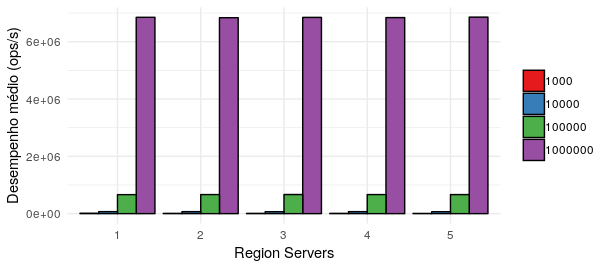
\includegraphics[width=\textwidth]{images/figura22}
        \caption{Latência}
        \label{figura22}
    \end{subfigure}
    \caption{\emph{Workload} 100\% scan variando o tamanho do conjunto de dados e o número de \emph{region servers} do \emph{cluster}.}
\end{figure*}

Pela análise dos resultados quanto ao desempenho médio dos testes da~\emph{workload} 100\%~\emph{read}/modify/write~--~Figura~\ref{figura19}, observou-se novamente que, a escalabilidade horizontal é mais evidenciada nos cenários onde o conjunto é igual a 1.000.000 de registros, sendo o desempenho médio dos testes com 5~\emph{region servers} maior que os resultados dos testes com 4, 3, 2 e 1~\emph{region servers} aproximadamente 4,5\%, 14,5\%, 29,7\% e 58,6\% respectivamente. Para os testes onde os conjuntos de dados foram iguais a 100.000 registros obteve-se nas execuções com 5~\emph{region servers} um desempenho médio maior que os testes com 4, 3, 2 e 1 \emph{region server} de aproximadamente 5,6\%, 7,1\%, 20,1\% e 47,7\% respectivamente.

Os testes onde os conjuntos de dados foram iguais a 1.000 registros não tiveram alterações significativas no desempenho médio, sendo a variação mais expressiva de menos de 6\% aumentando de 1 para 2 \emph{region servers}. Para o conjunto de 10.000 registro, a variação mais expressiva foi de aproximadamente 18,5\% quando aumentado de 1 para 2 \emph{region servers}. As demais adições de nós apresentaram uma variação de menos de 4\%.

Considerando os resultados dos testes da~\emph{workload} 100\%~\emph{read/modify/write} quanto a latência~--~Figura~\ref{figura20}. Novamente, o comportamento da latência acompanha o comportamento do desempenho médio de maneira inversamente proporcional e portanto, os testes com 1.000.000 de registros e 5~\emph{region servers} obtiveram uma latência menor que os testes com 4, 3, 2 e 1~\emph{region servers} em aproximadamente 4,4\%, 14,4\%, 29,9\% e 58,7\% respectivamente. Do mesmo modo, os testes com 100.000 registros e 5 \emph{region servers} obtiveram uma latência menor que os testes com 4, 3, 2 e 1 \emph{region servers} em aproximadamente 2,6\%, 7,7\%, 20,1\% e 47,9\% respectivamente.

Os testes da~\emph{workload} 100\%~\emph{read/modify/write} em que os conjuntos de dados foram iguais a 1.000 e 10.000 registros não tiveram alterações significativas na latência, seguindo a mesma porcentagem calculada nos testes de desempenho médio. Considerando os resultados dos testes da~\emph{workload} 100\%~\emph{scan} referentes ao desempenho médio~--~Figuras~\ref{figura21} e latência -- Figura~\ref{figura22}. Exceto nos testes cujos conjuntos de dados foram iguais a 1.000 registros, não houveram alterações significativas no desempenho médio do~\emph{cluster} sendo a variação mais expressiva de todos os conjuntos menor que 1,4\%. Portanto também não houve alteração significativa na latência em nenhum testes executados.

Para os testes cujo o conjunto de dados foi igual a 1.000 registros, o desempenho médio dos testes executados com 5~\emph{region servers} foi maior que do as execuções com 4, 3, 2 e 1~\emph{region servers} em aproximadamente 5,5\%, 2,4\%, 7\% e 42,5\% respectivamente. A latência das execuções com 5~\emph{region servers} foi menor que do as execuções com 4, 3, 2 e 1~\emph{region servers} em aproximadamente 5,3\%, 2,2\%, 6,5\% e 42\% respectivamente.

\section{Considerações Finais}
\label{sec:finais}

Este trabalho analisou a escalabilidade horizontal de um~\emph{cluster}  Hbase, submetendo o banco de dados a um \textit{benchmarking} apoiado pela ferramenta YSCB. Foram conduzidos testes com diferentes números de nós-escravos e tamanho do conjunto de dados.

Os resultados obtidos mostram que o escalonamento horizontal é mais evidente, considerando as~\emph{workloads} 100\%~\emph{write},~\emph{read} e~\emph{read/modify/write}, para conjuntos superiores a cem mil registros. Também foi identificado que o aumento do desempenho médio do~\emph{cluster} é mais significativo no aumento de~\emph{region servers} de 1 para 2 e de 2 para 3, sendo menos expressivos a partir de 3~\emph{region servers} (inferior a 8\%). Desta forma, a melhora no desempenho do~\emph{cluster} Hbase, considerando o desempenho médio e a latência das operações, é diretamente proporcional ao tamanho do conjunto de dados, de modo mais evidente.

O ganho de desempenho também varia de acordo com as operações realizadas no banco de dados. Por exemplo, o melhor aproveitamento do~\emph{cluster}  levando em conta o desempenho médio nas execuções com 5~\emph{region servers} foi alcançado pelos testes da~\emph{workload} 100\%~\emph{read}, sendo maior que os testes das~\emph{workloads} 100\%~\emph{write} e 100\%~\emph{read/modify/write} em aproximadamente 22\% e 28\% respectivamente. Contudo, os testes da~\emph{workload} 100\%~\emph{scan} mostraram que não há melhora no desempenho do~\emph{cluster}  para busca de registros, de modo independente do tamanho do conjunto de dados, devido a busca linear implementada pela ferramenta Hbase não ganhar eficiência a medida que novos nós são adicionados.

Os trabalhos futuros podem explorar o aumento do fator de replicação, não empregado neste trabalho, ao analisar o impacto que as operações adicionais de replicação podem causar à eficiência do~\emph{cluster}, considerando a inserção de novos nós.

\bibliographystyle{sbc}
\bibliography{sbc-template}

\end{document}